\section{Malware Classification}
\label{sec:ssdeep}

%Machine learning systems are just as good
%as the data they consumed. 
One potential use case of the massive amount of data 
available on \vt{} is to build 
machine learning models for applications
such as malware classifications and
clustering. In this section, we study
the question that {\em ``Is the data
provided by \vt{} enough to support
classifications and clusterings tasks?''}

Our study reveals both positive and
negative answers to this question.
Surprisingly, by just using the fuzzy hash strings of files submitted to \vt{},
we are able to build an automatic classifier whose
accuracy is higher than 80\% for some classification tasks
and we expect the quality to keep increasing
given more data.
Meanwhile, we identify some classification tasks
whose accuracy hardly beat random guesses.

To differentiate these cases and offer future researchers with more insights, 
we propose the use of a simple metrics to predict whether a given task belongs
the high-quality category or the low-quality
category. We hope our study shed lights
on future design of signatures for malware
detection.

%Malware detectors mainly rely on signatures manually extracted by security researchers. 
%ssdeep only takes static binary executable as inputs. 
%If we can build malware detector based on ssdeep similarity, 
%We can reduce or even eliminate manual efforts in malware detection. 


\subsection{Data Preparation}

\begin{table*}
  \centering
  \scriptsize
  {
  \begin{tabular}{clccc}
    \toprule
{\bf Index} & {\bf Microsoft Tag} & {\bf \# of Malwares} & {\bf \% of Tailing}  & {\bf \% of Distinct}\\
\midrule                                                                                                                                                                                                                                           
1  &  SoftwareBundler:Win32/Penzievs 	& 49380	     & 3.51\%  & 99.98\%\\
2  &  Adware:Win32/Hotbar               & 132161   & 1.88\%  & 99.98\%\\
3  &  TrojanDropper:Win32/Lamechi!rfn	& 39205	     & 0.01\%  & 6.13\%\\
4  &  Virus:Win32/Nabucur.D	            & 1190132  & 99.95\% & 100.00\%\\
5  &  Virus:Win32/Virut.BO	            & 84600	   & 21.84\% & 99.95\% \\
6  &  Worm:Win32/Mydoom.L@mm	        & 76259	     & 0\%     & 99.44\%\\
7  &  Virus:Win32/Ramnit.I              & 412052   & 3.07\%  & 96.76\%\\
8  &  Trojan:Win32/Dorv.A               & 54324    & 2.80\%  & 80.53\%\\
9  &  Trojan:Win32/Dynamer!ac           & 145402   & 65.17\% & 99.20\%\\
10 &  Virus:Win32/Ramnit.A              & 181524   & 26.79\% & 99.82\%\\   

\bottomrule
   \end{tabular}
   }
   \mycaption{tab:benchmark}{Benchmark Information.}
{\footnotesize{(Information for malwares used in our clustering and classification experiments. \# of Malwares: \# of distinct malwares we collected in each sampled malware group from 05/07/2016 to 09/06/2016. \% of Tailing: \% of tailing examples in each group. \% of Distinct: number of distinct ssdeep hash strings divided by group size.)}}
  %\nocaptionrule
  %\mycaption{tab:benchmark}{Malware Data Set.}
  %\footnotesize{(Information for malwares used in our clustering and classification experiments. \# of Malwares: \# of distinct malwares we collected in each sampled malware group from 05/07/2016 to 09/06/2016. \% of Tailing: \% of tailing examples for each group in the sampled 10000 malwares.)}
 %}
\end{table*}




Our study uses features based on ssdeep~\cite{ssdeep}, a program to compute fuzzy hashes. 
Specifically, ssdeep \yiying{fill here, what ssdeep exactly is and does}
Similarity between calculated hash strings can serve as an estimation for similarity between the two original files. 
\yiying{why can it estimate? we need some deeper understanding of the hash or need to be mroe careful when saying things like this. people's assumption is that hash cannot represent original data and is just a highly compressed string.}
\vt\ provides ssdeep hash strings as one of its metadata files and we collected them together with other metadata.

%We focus on classifying each malware into
%different malware families. 
We create training and testing
datasets using the detection results from Microsoft,
since Microsoft is more reliable in successfully detecting PE malwares~\cite{SongAPsys2016} than other anti-virus engines.
For each detected malware, 
Microsoft assigns a tag that contains type, platform, family, 
and variant information~\cite{microsoft}. 

We divide PE malwares detected by Microsoft engine into different groups, 
and malwares in the same group share the same Microsoft malware tag. 
We randomly sample 10 groups that have more than 10000 malwares.  
Table~\ref{tab:benchmark} presents the Microsoft tag sand the number of malwares in each sampled group we collected from \vt{}. 
Within each group, we randomly sample 10000 malwares and use these malwares in our classification and clustering experiments. 

\subsection{Classification Methodology and Results}
We use an API that \vt\ provides to compute the similarity between ssdeep string. \yiying{is the previous sentence correct?}
%ssdeep's compare API takes two ssdeep hash strings as inputs, 
%and return similarity between these two strings. 
We use 1 minus ssdeep similarity to get ssdeep distance.  

\subsubsection{KNN Classification}

We first use KNN~\cite{knn}, a simple classifier, to classify XXX.
KNN does ....
\yiying{full name of KNN, a simple description of it}
We design several experiments to understand the accuracy of 
the combination of KNN and ssdeep 
distance (or similarity) when handling different classification tasks. 

\noindent{\underline{\textit{Pair-wise two-class classification.}}}
We first build a two-class classifier for each of the 10 sampled groups. 
We use the 10000 sampled malwares in each group as positive examples (positive means being labeled as malware)
and randomly sample 10000 benign files as negative examples. 
Benign files are files submitted to \vt{} but are not labeled as malwares by any anti-virus engines. 
We randomly choose 5000 malwares and 5000 benign files for training and use the remaining files for testing.

We run cross validation for $k$ from 1 to 10 to pick up best $k$ value
and use the best $k$ value to test KNN using the testing set. 
Table~\ref{tab:benchmark} presents the best $k$ used for testing and classification results.
$k=1$ is always the best $k$ value for testing, except for two groups.

The classification accuracy of the two-class classifier differs in different groups.
For five out of ten malware groups, we achieve an accuracy higher than 80\%.
On the other hand, for
groups such as ``Virus:Win32/Nabucur.D'',
the classification accuracy is significantly lower. 
We get an accuracy of 59\% when
the accuracy of random guesses would be 50\%.
Overall, for the two-class classifier, 
there are not enough malwares and benign files in the training set to generate high-accuracy results. 

\noindent{\underline{\textit{Compelete ten-class classification.}}}
We also build a ten-class classifier.
We randomly choose 2000 malwares from each group and put half of them in the training set and the remaining half in the testing set. 
We run cross validation to pick up best $k$ from 1 to 10. 
The accuracy on the testing set with the best $k$ value 1 is 70.2\%. 

\begin{figure*}
\centering
\subfloat[Group 1]{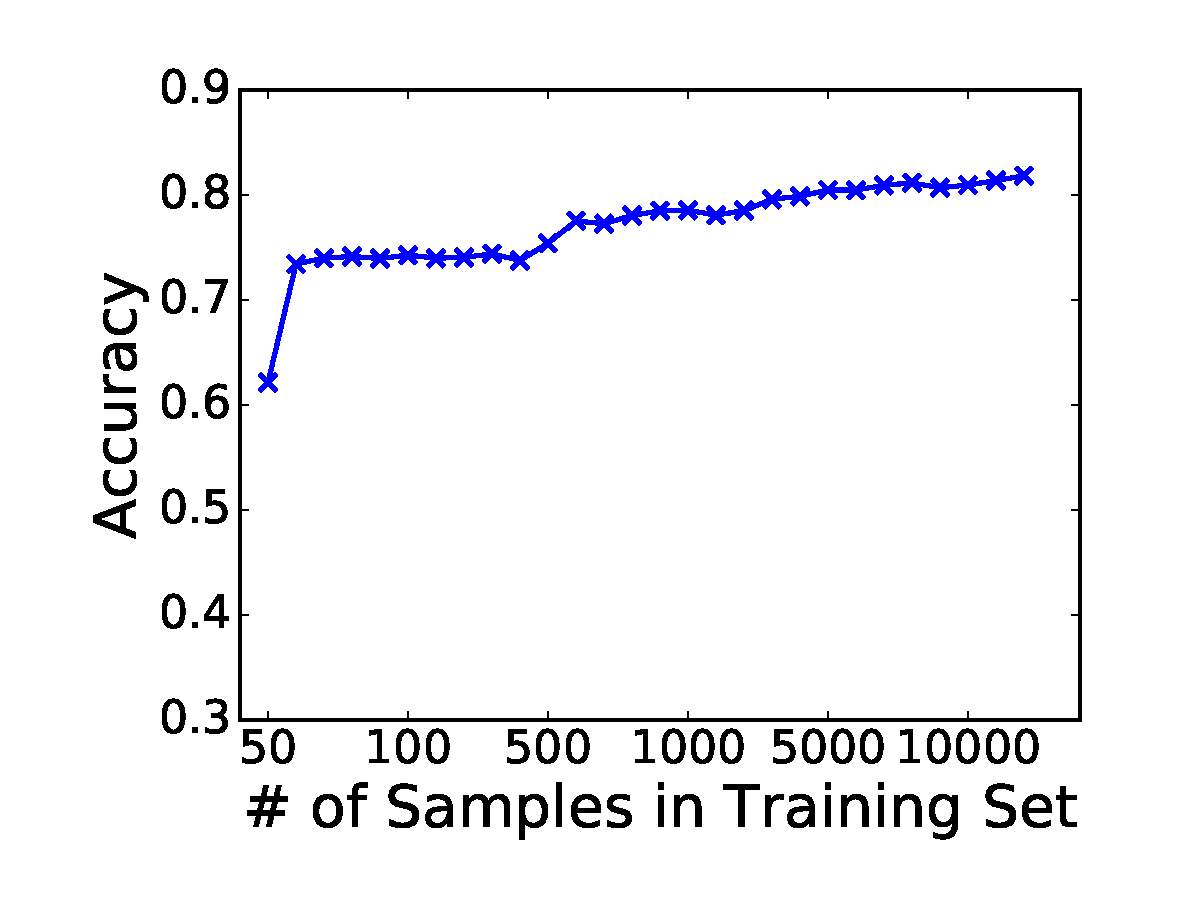
\includegraphics[width=0.16\linewidth]{figure/svm/0}\label{fig:moredata1}} 
\subfloat[Group 2]{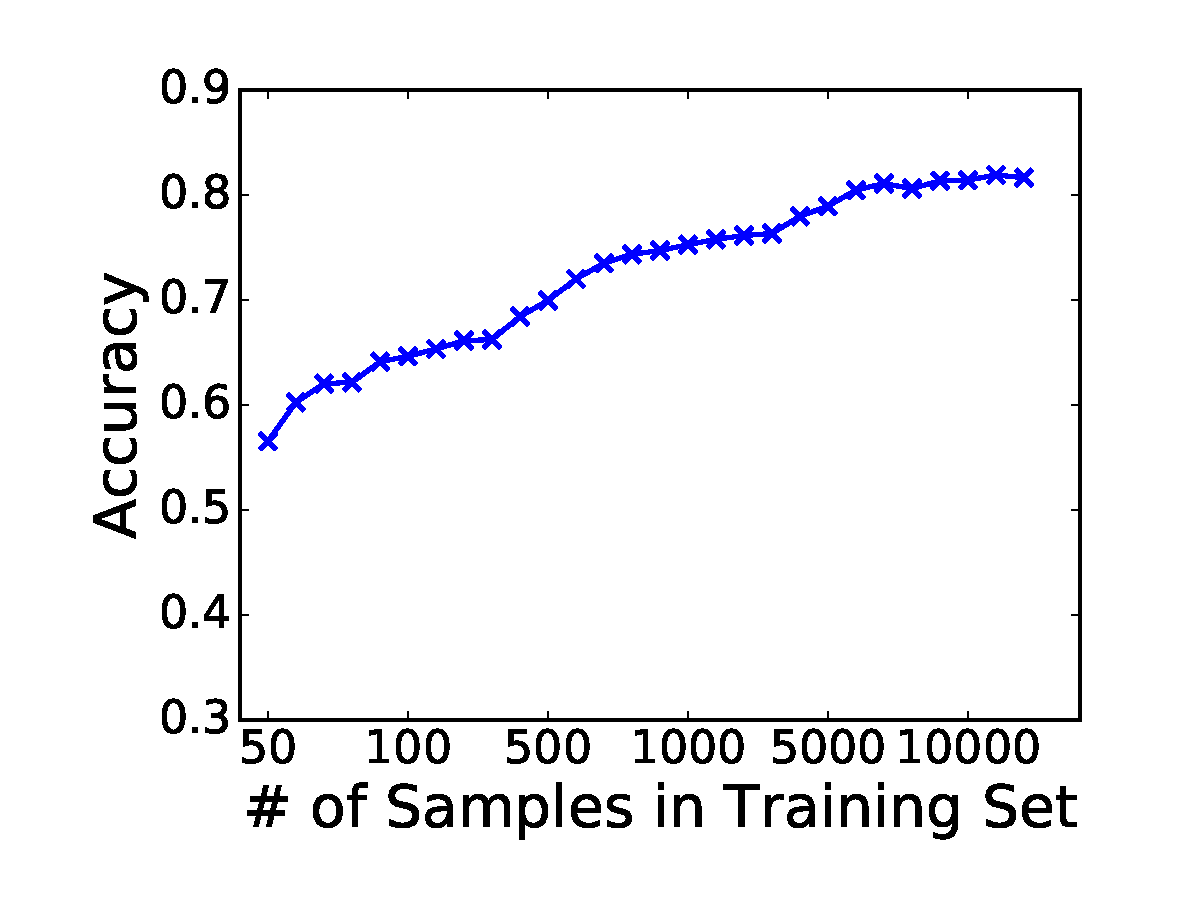
\includegraphics[width=0.16\linewidth]{figure/svm/1}\label{fig:moredata2}}
\subfloat[Group 3]{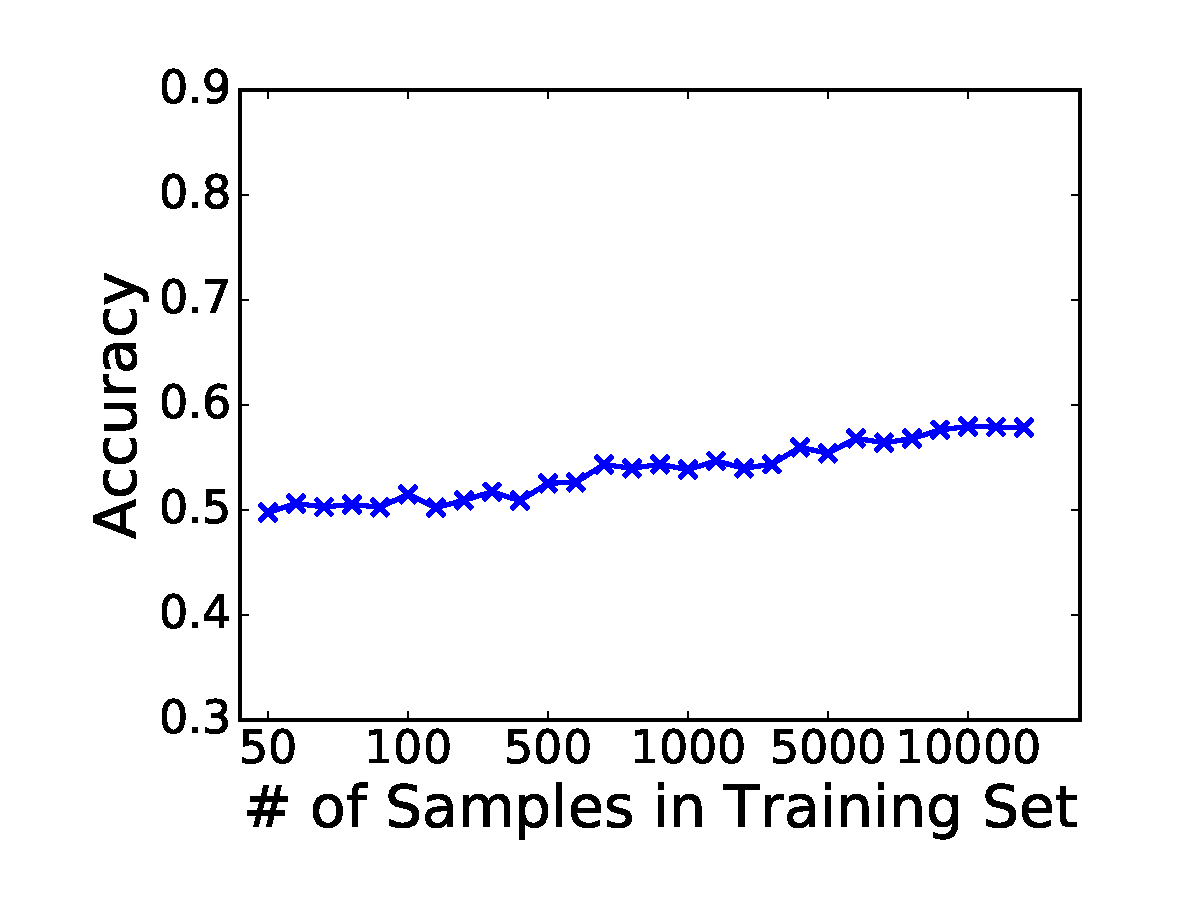
\includegraphics[width=0.16\linewidth]{figure/svm/2}\label{fig:moredata3}} 
\subfloat[Group 4]{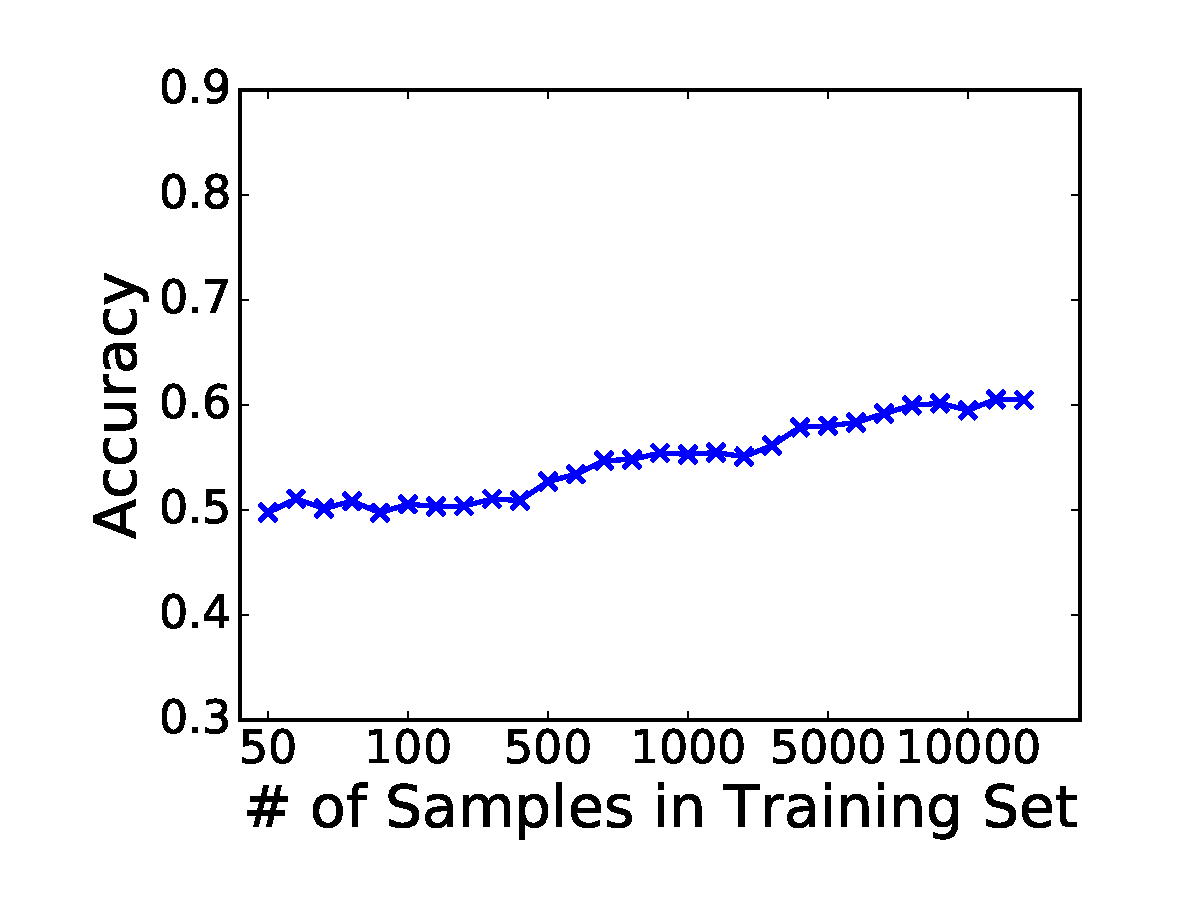
\includegraphics[width=0.16\linewidth]{figure/svm/3}\label{fig:moredata4}}
\subfloat[Group 5]{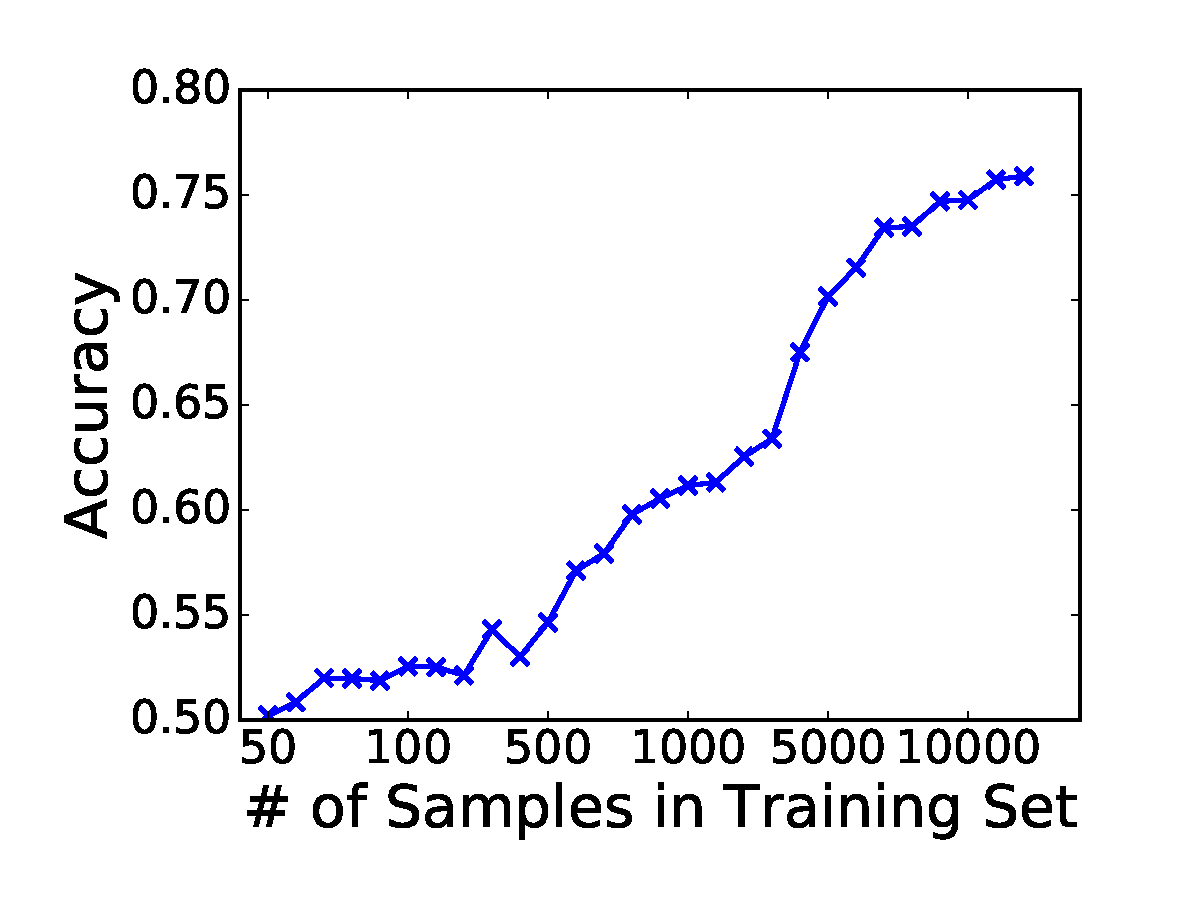
\includegraphics[width=0.16\linewidth]{figure/svm/4}\label{fig:moredata5}} \\ 

\subfloat[Group 6]{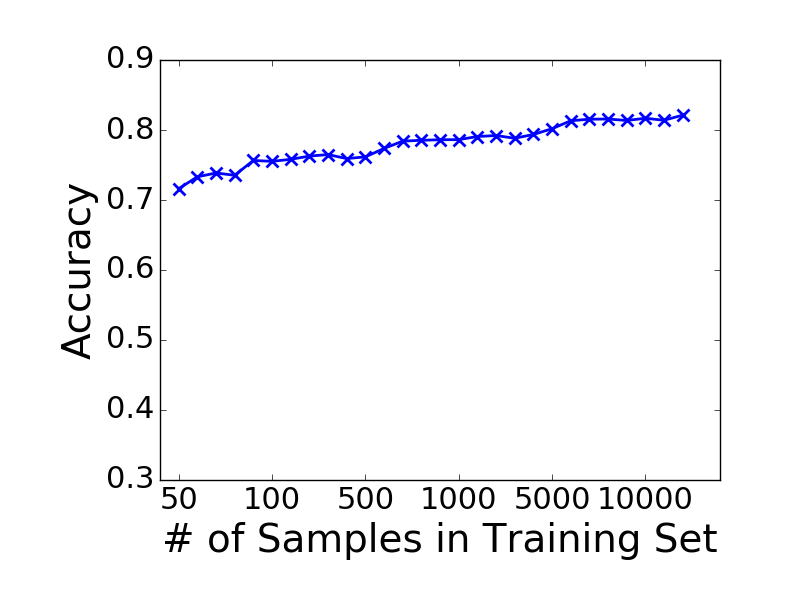
\includegraphics[width=0.16\linewidth]{figure/svm/5}\label{fig:moredata6}} 
\subfloat[Group 7]{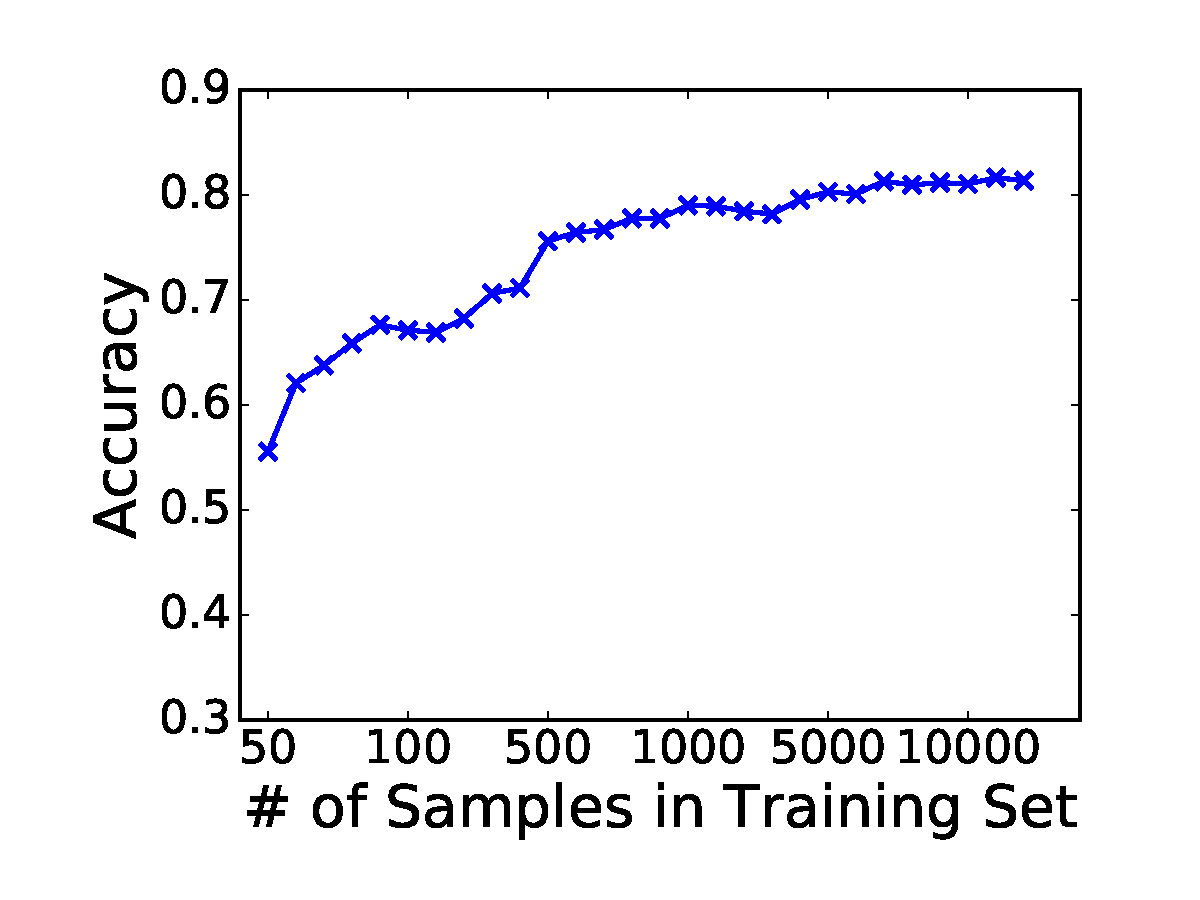
\includegraphics[width=0.16\linewidth]{figure/svm/6}\label{fig:moredata7}}
\subfloat[Group 8]{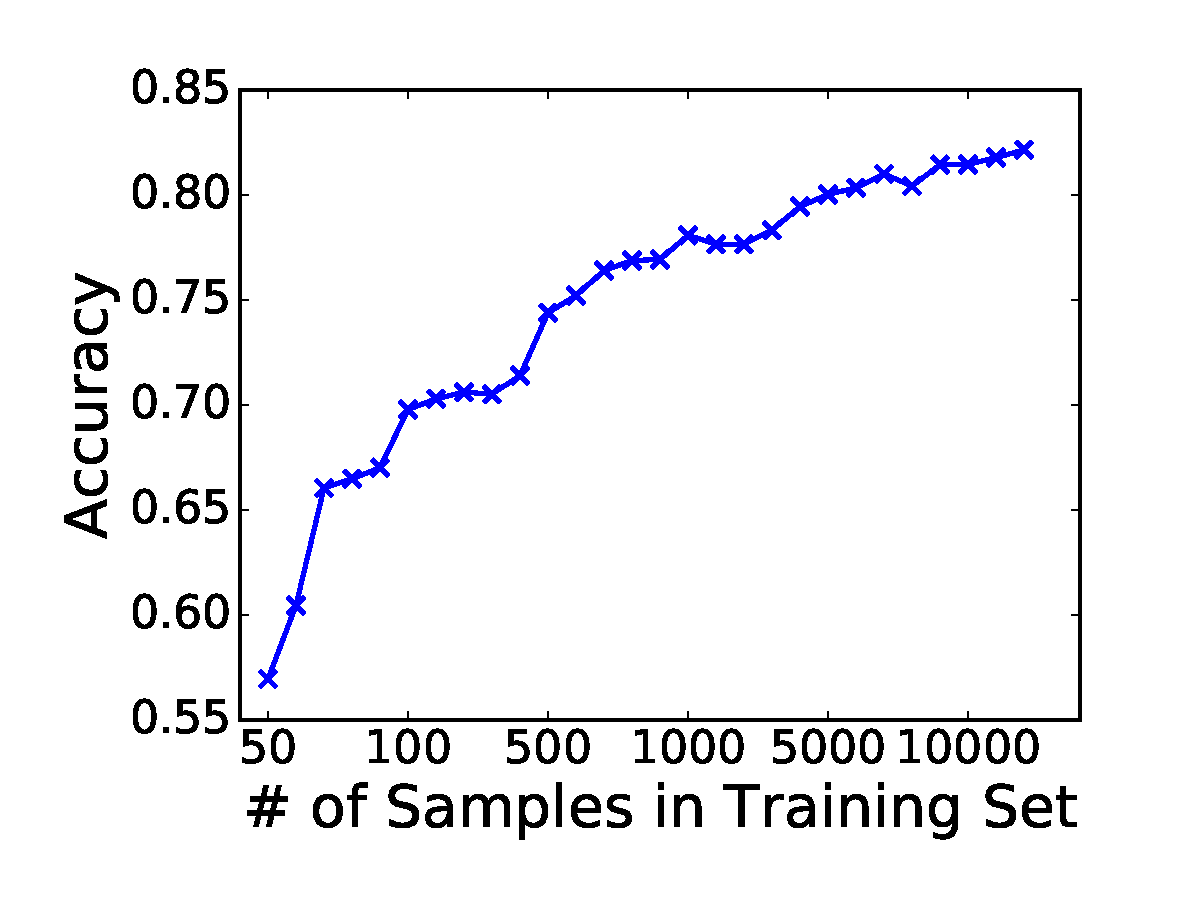
\includegraphics[width=0.16\linewidth]{figure/svm/7}\label{fig:moredata8}} 
\subfloat[Group 9]{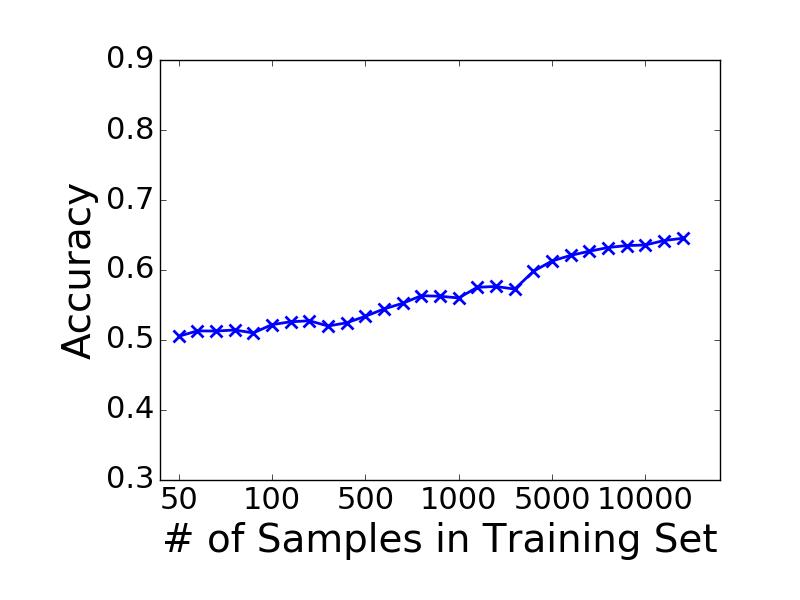
\includegraphics[width=0.16\linewidth]{figure/svm/8}\label{fig:moredata9}}
\subfloat[Group 10]{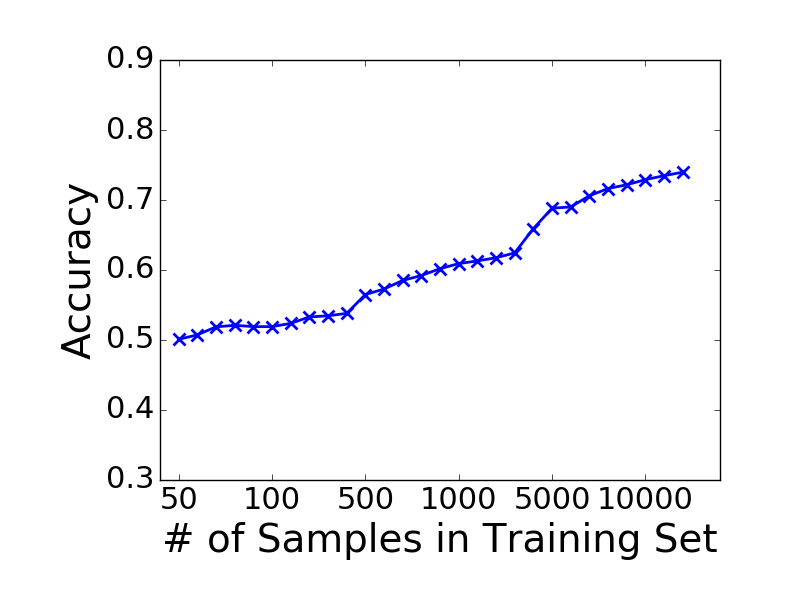
\includegraphics[width=0.16\linewidth]{figure/svm/9}\label{fig:moredata10}}
\subfloat[10-class]{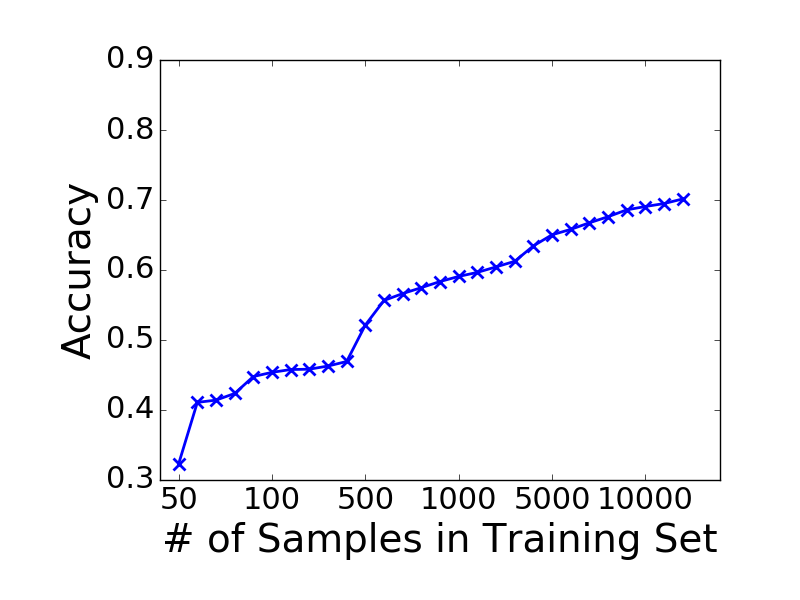
\includegraphics[width=0.16\linewidth]{figure/svm/10}\label{fig:moredata11}}
\caption{How accuracy changes with more data in traning set. 
{\footnotesize{(Figure~\ref{fig:moredata1} - Figure~\ref{fig:moredata10} show how accuracy of each two-class classifier changes 
with the size of training set changing from 50 to 10000. 
Figure~\ref{fig:moredata11} shows how accuracy of the ten-class classifier changes with the size of training set increaing from 50 to 10000. )}}} 
\label{fig:moredata} 
\end{figure*} 



\begin{figure}[t!]
\begin{center}
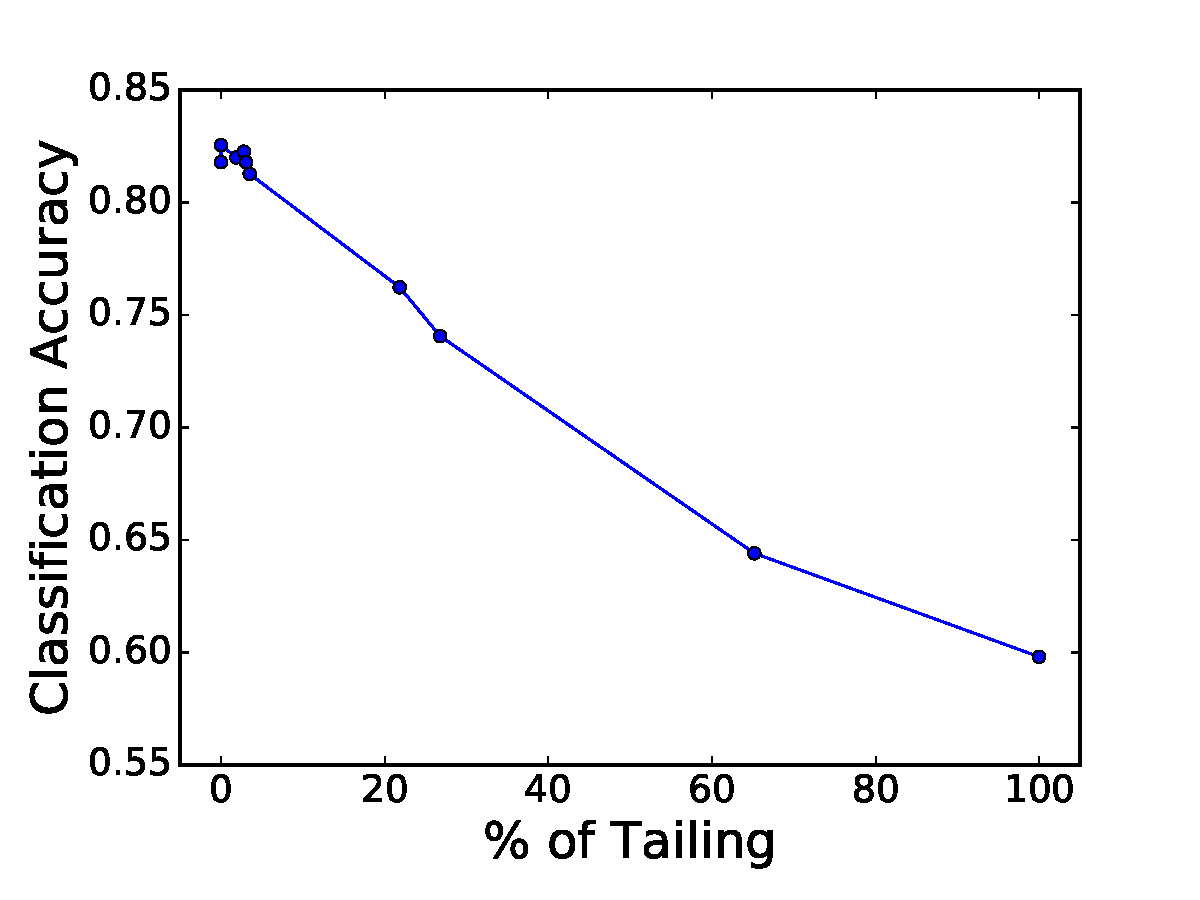
\includegraphics[width=2.5in]{figure/accuracy}
\mycaption{fig:accuracy}{The relation between classifer's accuracy and the percentage of tailing.}
{\footnotesize{(How classifier's accuracy changes with the percentage of tailing.)}}
\end{center}
%\vspace{-0.25in}
\end{figure}




\noindent{\underline{\textit{Effect of training set size.}}}
For each designed classifier, we further investigate 
how the size of training sets influences its accuracy.
We keep the test sets unchanged and increase the size of training sets from 50 to 10000.
%The total number of data points in all groups is the same.
We use the best $k$ value got from cross validation in earlier experiments.
Figure~\ref{fig:moredata} presents how accuracy changes with the size of training sets. 
As expected, for all classifiers, accuracy increases as there are more data in the training sets.
This constant increase in accuracy implies that with more data from \vt,
the classification accuracy is expected to be even higher.

\noindent{\underline{\textit{Classifications with semantics labels.}}}
To make classification based on more criteria, 
we further design a set of two-class classifications. 

First, we test the classfication of malwares with the same {\em class} but with different {\em variants} in the class.
Specifically, we classify malwares from Group 7 with malwares from Group 10. 
They are both from the same class ``Ramnit'', but in different variants. 
The accuracy we gotis 85.3\%. 

We then target to classify malwares in different {\em families}.
To do this, we classify malwares from Group 3 with malwares from Group 7 and Group 10
and classify malwares from Group 5 with malwares from Group 7 and Group 10. 
We get accuracies of 94.2\% and 85.8\%, respectively. 

Finally, we test the classification of different {\em types} of malware.
Specifically, we classify malwares from Group 8 and Group 9 with malwares from Group 4, Group 5, Group 7, and Group 10, 
the former groups have Trojan malwares and the latter group contains Virus. 
For this classification, we get 77.0\% accuracy. 
%We use the same experimental setting as previous two-class classifiers.  

{\bf Observation 9:}
{\em Different types of classification on \vt\ file ssdeep hash strings result in different accuracy, and increasing the training set size results in higher accuracy.}

\subsection{Tailing Malwares}
From the above study of various types of classification,
we find that using ssdeep hash strings to learn the similarities of \vt\ submission files 
is not always accurate.
But in some cases, the accuracy is very high.
To make use of these high-accuracy classification,
we need a good technique to seperate them from low-accuracy classification.

We identify a new metric to predict whether
a classification task falls into the
high-accuracy category or the low-accuracy
category. The intuition behind our idea is simple:
the ssdeep hash similarity of a data sample to other samples in the same group in
the training set is a proxy of the upper bound
of accuracy that we can expect. 
If no samples in a group are similar to each other, 
then no classifier can have high accuracy in predicting this class.
On the other hand, more similar samples will make it easy for a classifier to have high accuracy.

We call malwares that have no similarity with any other samples in the same group {\em tailing malwares}
and compute the percentage of tailing malwares in each group.
Table~\ref{tab:benchmark} lists the percentage of tailing malwares for each sampled group. 
Figure~\ref{fig:accuracy} plots the classification accuracy for all two-class classifiers against the percentage of tailing malwares.
The percentage of tailing malwares has a perfect linear relationship with classification accuracy,
implying that we can use tailing malware to predict the accuracy of a classifier.

{\bf Observation 10:} 
{\em The percentage of tailing malwares
can predict whether a given malware classification task is likely to have high or low accuracy.}

\begin{figure}[t!]
\begin{center}
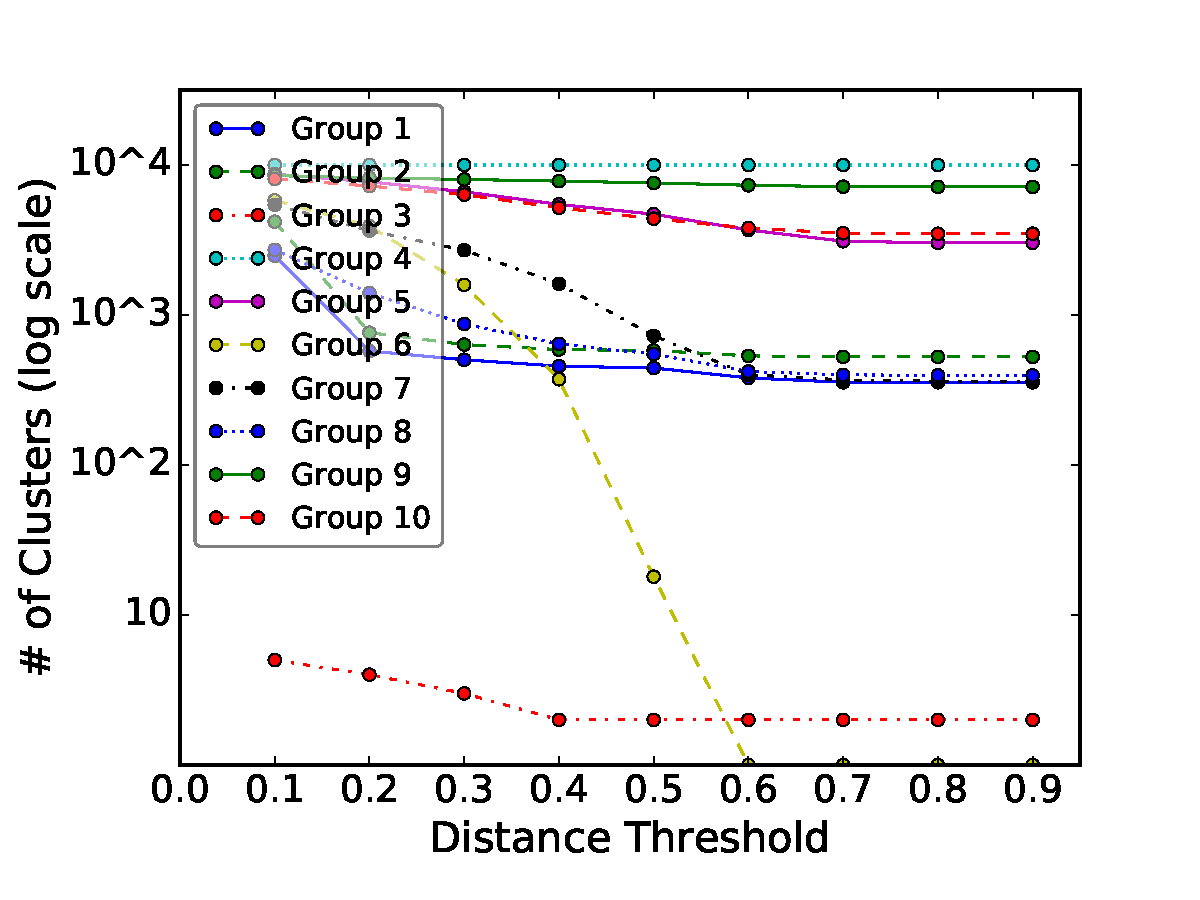
\includegraphics[width=2.5in]{figure/cluster}
\mycaption{fig:cluster}{The relation between resulting clusters and distance threshold.}
{\footnotesize{(How the number of resulting clusters change with different distance threshold.)}}
\end{center}
%\vspace{-0.25in}
\end{figure}


\subsection{SVM Classification}
%\noindent{\underline{\textit{SVM classification.}}}
Our previous experiments all used KNN as the classification algorithm.
We now discuss the potential of using
more sophisticated classifiers such as
support vector machines (SVM) on. 
SVM could take distance matrix as input,
but the size of the distance matrix is quadratic to the number of samples in the training set. 
\yiying{why is quadratic a problem? too big? cluster runs too slow?}
Nystrom methods~\cite{clustering-purpose} are popular ways to
approximate a distance matrix with clusters.
\yiying{is it cluster or classifier?}
Using Nystrom methods, each instance is transformed to a feature vector, where each dimension is the distance to a cluster center. 

\yiying{is it cluster or class? in all the discussion here you used cluster}
To understand the potential of applying Nystrom methods, we run hierarchical clustering~\cite{hcluster} on our data.
Hierarchical clustering starts with each instance as a cluster, 
and then it iteratively merges two clusters with minimum distance 
until distance threshold or cluster number threshold is reached. 
We use distance as threshold and the single linkage distance~\cite{single-link} as distance between two clusters. 

We change the distance threshold from 0.1 to 0.9
and count the resulting clusters under each experiment. 
Figure~\ref{fig:cluster} presents the experimental results.
As we increase the distance threshold, the number of resulting clusters decreases for each group. 
If we want to change a ssdeep hash string to a feature vector
based on distance of the string to the center of all clusters in training set, 
the size of the resulting feature vector would have a very large variance across different malware groups. 
This illustrates a challenge of directly applying
classic Nystrom method to our problem. 
However, we believe that it is possible to develop new approaches to
accommodate this observation.
\yiying{it's dangerous to say you believe some future work while you don't know what that future work is}

\yiying{Do we have any observation here?}

\subsection{Discussion}
\if 0
In our experiments, 1 is almost always the best k value. 
So using ssdeep similarity to conduct malware classification 
is roughly to search the most similar example in the training set for each testing example.
In our knn experiment, we compare a testing example with every example in training set. 
In the future, indexing techniques could be leveraged to reduce the complexity of identify 
the most similar example in training set from $O(n)$ to $O(1)$, where n is the number of examples in training set. 

Our experimental results show that with more data in training set, 
we can get better precision. 
For a testing instance, if there are similar instances in training set, 
classifier based on ssdeep similarity can precisely classify the instance. 
\fi

Our study found that by just using the ssdeep fuzzy hash string, 
we can achieve high accuracy in certain classification tasks, especially so with more data, 
and we developed a technique to predict when classification accuracy will be high.
The combination of these results point to one interesting direction for future researchers and security vendors, and to \vt:
instead of original files, we can use compressed representation of files to identify malwares.

With the ``big data'' available in the current world, we believe that this is a fruitful area to investigate.
The implication of this finding is significant. 
Users can have stronger privacy and do not need to submit, or reveal, their files to know if these files are likely to be malware.
%\vt{} contains huge amount of submitted files. We suggest \vt{} provides an extra API, 
%where users only need to submit ssdeep strings for suspicious files, 
%and this could improve privacy protection for \vt{}’s users.  



